\documentclass[professionalfonts, xcolor={usenames,svgnames,x11names,table}]{beamer}

\usetheme{HB}

\usepackage{tikz}
\usetikzlibrary{positioning}
\usetikzlibrary{shapes,backgrounds}
\usetikzlibrary{calc}

\usepackage{hanging}

\usepackage[utf8]{inputenc}	% not working with ð and þ; use \eth and \thorn instead
\usepackage[T1]{fontenc}	% scalable EC fonts
\usepackage{mathptmx}
\usepackage{amssymb, amsmath} % for symbols
\usepackage{tipa}

\usepackage{gb4e}

\newcommand{\subpoint}[1]{{small\color{LightSteelBlue4}#1}}
\colorlet{fhighlight}{orange}

\title[TSL SF]{%
    \texorpdfstring{Computational representation of unbounded stress: \\ tiers with structural features}%
    {Computational representation of unbounded stress: tiers with structural features}}
\author{%
    Hyunah Baek
}

\institute{Stony Brook University\\\texttt{hyunah.baek@stonybrook.edu}\\\texttt{}}
\date{Computational Phonology Workshop\\Dec 12, 2016}

\begin{document}
\unnumbered{
\begin{frame}
	\titlepage
\end{frame}
}

\unnumbered{
\begin{frame}{Take Home Message}
	\begin{itemize}
		\item Most phonological patterns fit into the class of \emph{tier-based strictly local} dependencies (TSL) (Heinz 2016).
		\item However, there still remain patterns that ostensibly display higher complexity than TSL\@, e.g., unbounded stress.
	\end{itemize}
	\pause
    \begin{block}{Tiers with structural features}
        Once grammar has access to structural information of syllables, unbounded stress patterns are TSL after all.
    \end{block}
\end{frame}
}

\unnumbered{
\begin{frame}{Outline}
   \tableofcontents
\end{frame}
}

\section[RHOL]{Unbounded stress: RHOL as TSL}

\begin{frame}{Unbounded stress: RHOL}
    \textbf{Chuvash word stress} (Hayes 1995)
    \vskip2em
    \hspace*{-8pt}\makebox[\linewidth][c]{%
    \begin{tabular}{ll}
    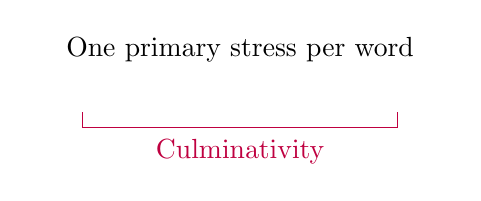
\begin{tikzpicture}
    \node at (2,0) {One primary stress per word};
    \node at (2,-0.5) {\phantom{otherwise on the leftmost syllable}};
    \draw<2>[purple] (0,-0.8) -- (0,-1) -- (4,-1) -- (4,-0.8);
    %\draw<2->[dotted, thick, red] (-0.25,0) to (-1,0);
    \node at (2,-1.3) {\phantom{Culminativity}};
    \node<2-> at (2,-1.3) {\textcolor{purple}{Culminativity}};
    \end{tikzpicture}
    &
    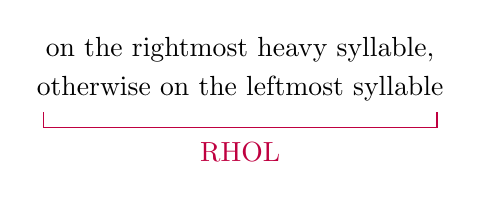
\begin{tikzpicture}
    \node at (2.5,0) {on the rightmost heavy syllable,};
    \node at (2.5,-0.5) {otherwise on the leftmost syllable};
	\draw<2>[purple] (0,-0.8) -- (0,-1) -- (5,-1) -- (5,-0.8);
	\node at (2.5,-1.3) {\phantom{RHOL}};
	\node<2-> at (2.5,-1.3) {\textcolor{purple}{RHOL}};
	\end{tikzpicture}\\
	\end{tabular}
	}
    \vskip 2em
    \hspace*{-8pt}\makebox[\linewidth][c]{%
    {\renewcommand{\arraystretch}{1.3}
    \begin{tabular}{c|c}
    \hline
    well-formed & ill-formed \\
    \hline
    LH\'H & $^{*}$\'LH\'H \\
    L\'HL & $^{*}$L\'HH \\
    \'LLL & $^{*}$LL\'L \\
    \hline
    \end{tabular}
    }}
\end{frame}


\begin{frame}{Culminativity}
    Culminativity: Every word has exactly one primary stress
    \vskip 1em
    \begin{block}{Culminativity is Tier-based Strictly Local (TSL)}
        \vskip 0.5em
        $
		G= \left \langle T = \{\text{\alert<2-3>{\'H, \'L, $\rtimes$, $\ltimes$}}\}, \quad S = \{\text{\alert<4>{$^{*}$\'H\'H, $^{*}$\'L\'L, $^{*}$\'H\'L, $^{*}$\'L\'H, $^{*}$$\rtimes$$\ltimes$}}\} \right \rangle
		$
		\vskip 0.5em
    \end{block}

    \vskip 1em
%Culminativity examples: (a) licit, (b-c) illicit
	\small
	\begin{minipage}{.32\textwidth}
	a.
	\end{minipage}
	%
	\begin{minipage}{.32\textwidth}
	b.
	\end{minipage}
	%
	\begin{minipage}{.32\textwidth}
	c.
	\end{minipage}

	\begin{minipage}{.32\textwidth}
	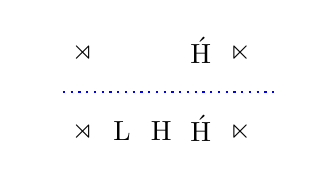
\begin{tikzpicture}[baseline]
	\node (-1) at (-0.5,0) {\phantom{$^{*}$}};
	\node (0) at (0,0) {$\rtimes$};
	\node (1) at (0.5,0) {L};
	\node (2) at (1,0) {H};
	\node (3) at (1.5,0.03) {\'H};
	\node (4) at (2,0) {$\ltimes$};

    \draw<2->[dotted, thick, blue] (-0.25,0.5) to (2.5,0.5);
    %\node at (-0.5,0.7) {{\tiny Tier}};

    \begin{scope}
        %+
        \node<3-> (00) at (0,1) {$\rtimes$};
        \node<3-> (03) at (1.5,1.03) {\'H};
        \node<3-> (04) at (2,1) {$\ltimes$};
        \draw<-3>[dashed, white] (0.3,0.7) -- (1.7,0.7) -- (1.7,1.3) -- (0.3,1.3) -- (0.3,0.7);
    \end{scope}
	\end{tikzpicture}
	\end{minipage}
	%
	\begin{minipage}{.32\textwidth}
	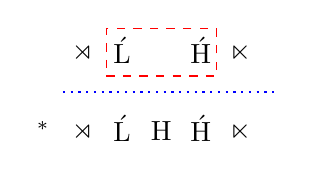
\begin{tikzpicture}[baseline]
	\node (-1) at (-0.5,0) {$^{*}$};
	\node (0) at (0,0) {$\rtimes$};
	\node (1) at (0.5,0.03) {\'L};
	\node (2) at (1,0) {H};
	\node (3) at (1.5,0.03) {\'H};
	\node (4) at (2,0) {$\ltimes$};

    \draw<2->[dotted, thick, blue] (-0.25,0.5) to (2.5,0.5);
    %\node at (-0.5,0.7) {{\tiny Tier}};

    \begin{scope}
        %+
        \node<3-> (00) at (0,1) {$\rtimes$};
        \node<3-> (01) at (0.5,1.03) {\'L};
        \node<3-> (03) at (1.5,1.03) {\'H};
        \node<3-> (04) at (2,1) {$\ltimes$};
        \draw<-3>[dashed, white] (0.3,0.7) -- (1.7,0.7) -- (1.7,1.3) -- (0.3,1.3) -- (0.3,0.7);
        \draw<4>[dashed, red] (0.3,0.7) -- (1.7,0.7) -- (1.7,1.3) -- (0.3,1.3) -- (0.3,0.7);
    \end{scope}
	\end{tikzpicture}
	\end{minipage}
	%
	\begin{minipage}{.32\textwidth}
	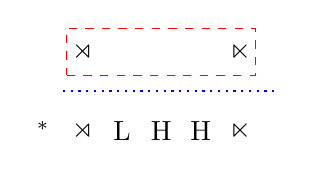
\begin{tikzpicture}[baseline]
	\node (-1) at (-0.5,0) {$^{*}$};
	\node (0) at (0,0) {$\rtimes$};
	\node (1) at (0.5,0) {L};
	\node (2) at (1,0) {H};
	\node (3) at (1.5,0) {H};
	\node (4) at (2,0) {$\ltimes$};

    \draw<2->[dotted, thick, blue] (-0.25,0.5) to (2.5,0.5);
    %\node at (-0.5,0.7) {{\tiny Tier}};

    \begin{scope}
        %+
        \node<3-> (01) at (0,1) {$\rtimes$};
        \node<3-> (04) at (2,1) {$\ltimes$};
        \draw<-3>[dashed, white] (0.3,0.7) -- (1.7,0.7) -- (1.7,1.3) -- (0.3,1.3) -- (0.3,0.7);
        \draw<4>[dashed, red] (-0.2,0.7) -- (2.2,0.7) -- (2.2,1.3) -- (-0.2,1.3) -- (-0.2,0.7);
    \end{scope}
	\end{tikzpicture}
	\end{minipage}
\end{frame}



\begin{frame}{RHOL}
    RHOL: Rightmost heavy, otherwise leftmost
    \vskip 1em
    \begin{block}{RHOL is TSL}
        \vskip 0.5em
        $
		G= \left \langle T = \{\text{\'H, H, \'L, L}\}, \quad S = \{\text{$^{*}$\'HH, $^{*}$\'LH, $^{*}$H\'L, $^{*}$L\'L}\} \right \rangle
		$
		\vskip 0.5em
    \end{block}

    \vskip 1em
    \begin{minipage}{.32\textwidth}
	a.
	\end{minipage}
	%
	\begin{minipage}{.32\textwidth}
	b.
	\end{minipage}
	%
	\begin{minipage}{.32\textwidth}
	c.
	\end{minipage}

    \begin{minipage}{.32\textwidth}
	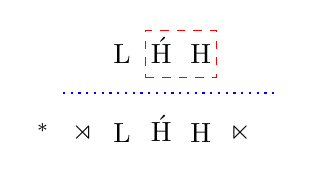
\begin{tikzpicture}[baseline]
	\node (-1) at (-0.5,0) {$^{*}$};
	\node (0) at (0,0) {$\rtimes$};
	\node (1) at (0.5,0) {L};
	\node (2) at (1,0.05) {\'H};
	\node (3) at (1.5,0) {H};
	\node (4) at (2,0) {$\ltimes$};

    \draw<2>[dotted, thick, blue] (-0.25,0.5) to (2.5,0.5);
    %\node at (-0.5,0.7) {{\tiny Tier}};

    \begin{scope}
        %+
        \node<2> (01) at (0.5,1) {L};
        \node<2> (02) at (1,1.05) {\'H};
        \node<2> (03) at (1.5,1) {H};
        \draw<1>[dashed, white] (0.3,0.7) -- (1.7,0.7) -- (1.7,1.3) -- (0.3,1.3) -- (0.3,0.7);
  		\draw<2>[dashed, red] (0.8,0.7) -- (1.7,0.7) -- (1.7,1.3) -- (0.8,1.3) -- (0.8,0.7);
    \end{scope}
	\end{tikzpicture}
\end{minipage}
%
\begin{minipage}{.32\textwidth}
	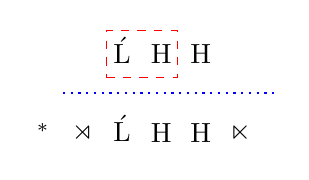
\begin{tikzpicture}[baseline]
	\node (-1) at (-0.5,0) {$^{*}$};
	\node (0) at (0,0) {$\rtimes$};
	\node (1) at (0.5,0.05) {\'L};
	\node (2) at (1,0) {H};
	\node (3) at (1.5,0) {H};
	\node (4) at (2,0) {$\ltimes$};

    \draw<2>[dotted, thick, blue] (-0.25,0.5) to (2.5,0.5);
    %\node at (-0.5,0.7) {{\tiny Tier}};

    \begin{scope}
        %+
        \node<2> (01) at (0.5,1.05) {\'L};
        \node<2> (02) at (1,1) {H};
        \node<2> (03) at (1.5,1) {H};
        \draw<1>[dashed, white] (0.3,0.7) -- (1.7,0.7) -- (1.7,1.3) -- (0.3,1.3) -- (0.3,0.7);
        \draw<2>[dashed, red] (0.3,0.7) -- (1.2,0.7) -- (1.2,1.3) -- (0.3,1.3) -- (0.3,0.7);
    \end{scope}
	\end{tikzpicture}
\end{minipage}
%
\begin{minipage}{.32\textwidth}
	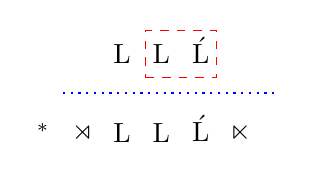
\begin{tikzpicture}[baseline]
	\node (-1) at (-0.5,0) {$^{*}$};
	\node (0) at (0,0) {$\rtimes$};
	\node (1) at (0.5,0) {L};
	\node (2) at (1,0) {L};
	\node (3) at (1.5,0.05) {\'L};
	\node (4) at (2,0) {$\ltimes$};

    \draw<2>[dotted, thick, blue] (-0.25,0.5) to (2.5,0.5);
    %\node at (-0.5,0.7) {{\tiny Tier}};

    \begin{scope}
        %+
        \node<2> (01) at (0.5,1) {L};
		\node<2> (02) at (1,1) {L};
		\node<2> (03) at (1.5,1.05) {\'L};
		\draw<1>[dashed, white] (0.3,0.7) -- (1.7,0.7) -- (1.7,1.3) -- (0.3,1.3) -- (0.3,0.7);
        \draw<2>[dashed, red] (0.8,0.7) -- (1.7,0.7) -- (1.7,1.3) -- (0.8,1.3) -- (0.8,0.7);
    \end{scope}
	\end{tikzpicture}
\end{minipage}
\vskip 0.5em
\end{frame}




\section[non-final RHOL]{Non-final RHOL as TSL?}

\begin{frame}{Unbounded stress: Non-final RHOL}
    \textbf{Classical Arabic word stress} (McCarthy 1979)
    \vskip2em
    \hspace*{-8pt}\makebox[\linewidth][c]{%
    \begin{tabular}{ll}
    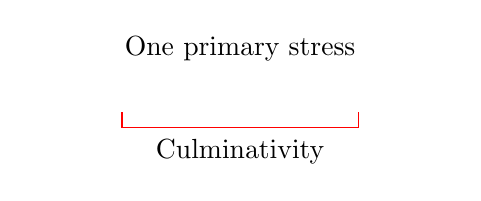
\begin{tikzpicture}
    \node at (1.5,0) {One primary stress};
    \node at (1.5,-0.5) {\phantom{otherwise on the leftmost syllable}};
    \draw<2>[red] (0,-0.8) -- (0,-1) -- (3,-1) -- (3,-0.8);
    %\draw<2->[dotted, thick, red] (-0.25,0) to (-1,0);
    \node<1> at (1.5,-1.3) {\phantom{Culminativity}};
    \node<2-> at (1.5,-1.3) {\alert{Culminativity}};
    \end{tikzpicture}
    &
    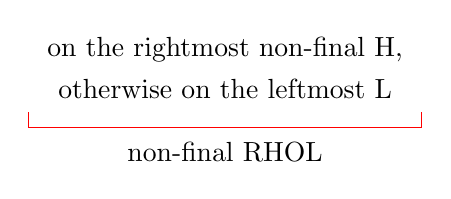
\begin{tikzpicture}
    \node at (2.5,0) {on the rightmost non-final H,};
    \node at (2.5,-0.5) {otherwise on the leftmost L};
	\draw<2>[red] (0,-0.8) -- (0,-1) -- (5,-1) -- (5,-0.8);
	\node<1> at (2.5,-1.3) {\phantom{non-final RHOL}};
	\node<2-> at (2.5,-1.3) {\alert{non-final RHOL}};
	\end{tikzpicture}\\
	\end{tabular}
	}
	\vskip 2em
    \hspace*{-8pt}\makebox[\linewidth][c]{%
    {\renewcommand{\arraystretch}{1.3}
    \begin{tabular}{c|c}
    \hline
    well-formed & ill-formed \\
    \hline
    LL\'HH & $^{*}$LLH\'H \\
    LH\'HH & $^{*}$L\'HHH \\
    \'LLLL & $^{*}$LLL\'L \\
    \hline
    \end{tabular}
    }}
\end{frame}



\begin{frame}{Non-final RHOL as TSL?}
    Non-final RHOL: Non-final rightmost H, otherwise leftmost
    \vskip 1em
    \begin{block}{Is Non-final RHOL TSL?}
        \vskip 0.5em
        $
        G= \left \langle T= \{\text{\'H, H, \'L, \alert<1>{$\ltimes$}}\}, \quad S = \{\text{\alert<1>{$^{*}$\'H$\ltimes$}, \alert<2-3>{$^{*}$\'HH}, $^{*}$\'LH, $^{*}$H\'L, $^{*}$L\'L}\} \right\rangle
        $
		\vskip 0.5em
    \end{block}
    \vskip 2em
	\small
	\hspace*{-10pt}\makebox[\linewidth][c]{%
	\begin{minipage}{.35\textwidth}
	a.
	\end{minipage}
	%
	\begin{minipage}{.32\textwidth}
	b.
	\end{minipage}
	%
	\begin{minipage}{.3\textwidth}
	c.
	\end{minipage}
	}
	\hspace*{-10pt}\makebox[\linewidth][c]{%
	\begin{minipage}{.35\textwidth}
	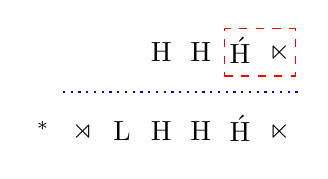
\begin{tikzpicture}[baseline]
	\node (-1) at (-0.5,0) {$^{*}$};
	\node (0) at (0,0) {$\rtimes$};
	\node (1) at (0.5,0) {L};
	\node (2) at (1,0) {H};
	\node (3) at (1.5,0) {H};
	\node (4) at (2,0.03) {\'H};
	\node (6) at (2.5,0) {$\ltimes$};

    \draw[dotted, thick, blue] (-0.25,0.5) to (2.75,0.5);
    %\node at (-0.5,0.7) {{\tiny Tier}};

    \begin{scope}
        %+
		\node (02) at (1,1) {H};
		\node (03) at (1.5,1) {H};
		\node (04) at (2,1.03) {\'H};
		\node (06) at (2.5,1) {$\ltimes$};
		\draw[dashed, red] (1.8,0.7) -- (2.7,0.7) -- (2.7,1.3) -- (1.8,1.3) -- (1.8,0.7);
    \end{scope}
	\end{tikzpicture}
	\end{minipage}
	%
	\begin{minipage}{.32\textwidth}
	\pause
	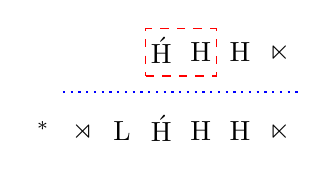
\begin{tikzpicture}[baseline]
	\node (-1) at (-0.5,0) {$^{*}$};
	\node (0) at (0,0) {$\rtimes$};
	\node (1) at (0.5,0) {L};
	\node (2) at (1,0.03) {\'H};
	\node (3) at (1.5,0) {H};
	\node (4) at (2,0) {H};
	\node (6) at (2.5,0) {$\ltimes$};

    \draw[dotted, thick, blue] (-0.25,0.5) to (2.75,0.5);
    %\node at (-0.5,0.7) {{\tiny Tier}};

    \begin{scope}
        %+
		\node (02) at (1,1.03) {\'H};
		\node (03) at (1.5,1) {H};
		\node (04) at (2,1) {H};
		\node (06) at (2.5,1) {$\ltimes$};
		\draw[dashed, red] (0.8,0.7) -- (1.7,0.7) -- (1.7,1.3) -- (0.8,1.3) -- (0.8,0.7);

    \end{scope}
	\end{tikzpicture}
	\end{minipage}
	%
	\begin{minipage}{.3\textwidth}
	\pause
	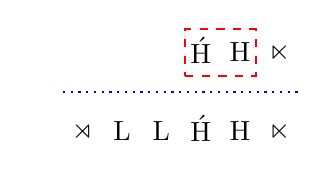
\begin{tikzpicture}[baseline]
	\node (-1) at (-0.5,0) {\phantom{$^{*}$}};
	\node (0) at (0,0) {$\rtimes$};
	\node (1) at (0.5,0) {L};
	\node (2) at (1,0) {L};
	\node (3) at (1.5,0.03) {\'H};
	\node (4) at (2,0) {H};
	\node (6) at (2.5,0) {$\ltimes$};

    \draw[dotted, thick, blue] (-0.25,0.5) to (2.75,0.5);
    %\node at (-0.5,0.7) {{\tiny Tier}};

    \begin{scope}
        %+
        \node (03) at (1.5,1.03) {\'H};
		\node (04) at (2,1) {H};
		\node (06) at (2.5,1) {$\ltimes$};
        \draw[dashed, thick, red] (1.3,0.7) -- (2.2,0.7) -- (2.2,1.3) -- (1.3,1.3) -- (1.3,0.7);
    \end{scope}
	\end{tikzpicture}
	\end{minipage}
	}
\vskip 2em
\pause
Without a distinction between \alert{final and non-final H}, TSL approaches over-\slash under-generate.

\end{frame}

\section[TSL-SF]{TSL with Structural Features}

\subsection{Tiers with Structural Features}
\begin{frame}{Structural Features}
    Prosodic elements are composed of structural features.\\
    (e.g., syllable weight, stress, syllable location, word boundary)
    \pause
    \vskip 2em
	\small
	\hspace*{-2pt}\makebox[\linewidth][c]{%
	{\renewcommand{\arraystretch}{1.3}
	\begin{tabular}{cccccc}
	$\rtimes$ & L & L & \'H & H & $\ltimes$\\
	\hline
	+boundary & +light & +light & +heavy & +heavy & +boundary \\[-2pt]
	& -stress & -stress & +stress & -stress & \\[-2pt]
	& +initial & -initial & -initial & -initial & \\[-2pt]
	& -final & -final & -final & +final & \\
	\end{tabular}}}
	\vskip 2em
	%These features rather than whole syllables trigger tier projection. 
\end{frame}

\subsection{Non-final RHOL as TSL-SF}
\begin{frame}{Tier-based Strictly Local with Structural Features (TSL-SF)}
	\begin{block}{Non-final RHOL is TSL-SF}
        \vskip 0.5em
        \small
        $
        G= \left \langle T = \begin{Bmatrix}
		[\text{+stress}], \\ [\text{+heavy}],\\ [\text{+initial}], \\ [\text{+final}] 
		\end{Bmatrix}
		, \quad S = \begin{Bmatrix}
		\text{$^{*}$[+heavy,+stress,-initial,+final]}, \\ 
		\text{$^{*}$[+light,+stress,-initial]}, \\
		\text{$^{*}$[+heavy,+stress][+heavy,-stress,-final]}, \\
		\text{$^{*}$[+light,+stress][+heavy,-stress,-final]}
		\end{Bmatrix} \right \rangle
        $
		\vskip 0.5em
    \end{block}
	\vskip 1em
	\begin{itemize}
		\item \textit{T} specifies feature matrices such that a symbol is projected onto the tier iff it is compatible with one of the matrices.
		\item \textit{S} specifies forbidden substrings that must not be present in strings projected on the tier.
	\end{itemize}
\end{frame}

\begin{frame}{Tier-based Strictly Local with Structural Features (TSL-SF)}
		\begin{block}{Non-final RHOL is TSL-SF}
		\vskip 0.5em
        \small
        $
        G= \left \langle T = \begin{Bmatrix}
		[\text{+stress}], \\ [\text{+heavy}],\\ [\text{+initial}], \\ [\text{+final}] 
		\end{Bmatrix}
		, \quad S = \begin{Bmatrix}
		\text{$^{*}$[+heavy,+stress,-initial,+final]}, \\ 
		\text{$^{*}$[+light,+stress,-initial]}, \\
		\text{\alert<3>{$^{*}$[+heavy,+stress][+heavy,-stress,-final]}}, \\
		\text{$^{*}$[+light,+stress][+heavy,-stress,-final]}
		\end{Bmatrix} \right \rangle
        $
		\vskip 0.5em
    \end{block}
	\vskip 1em
	\small
	\hspace*{3pt}\makebox[\linewidth][c]{%
	\begin{minipage}{.5\textwidth}
	a.
	\end{minipage}
	\begin{minipage}{.4\textwidth}
	b.
	\end{minipage}
	}
	\hspace*{3pt}\makebox[\linewidth][c]{%
	\begin{minipage}{.5\textwidth}
	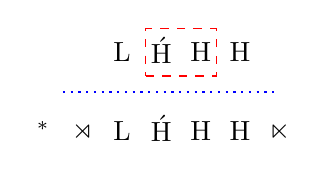
\begin{tikzpicture}[baseline]
	\node (-1) at (-0.5,0) {$^{*}$};
	\node (0) at (0,0) {$\rtimes$};
	\node (1) at (0.5,0) {L};
	\node (2) at (1,0.03) {\'H};
	\node (3) at (1.5,0) {H};
	\node (4) at (2,0) {H};
	\node (6) at (2.5,0) {$\ltimes$};

    \draw<2->[dotted, thick, blue] (-0.25,0.5) to (2.5,0.5);
    %\node at (-0.5,0.7) {{\tiny Tier}};

    \begin{scope}
        %+
        \node (01) at (0.5,1) {\phantom{L}};
        \node<2-> (01) at (0.5,1) {L};
		\node<2-> (02) at (1,1.03) {\'H};
		\node<2-> (03) at (1.5,1) {H};
		\node<2-> (04) at (2,1) {H};
		\draw<2->[dashed, red] (0.8,0.7) -- (1.7,0.7) -- (1.7,1.3) -- (0.8,1.3) -- (0.8,0.7);

    \end{scope}
	\end{tikzpicture}
	\end{minipage}
	%
	\begin{minipage}{.4\textwidth}
	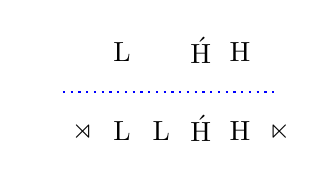
\begin{tikzpicture}[baseline]
	\node (-1) at (-0.5,0) {\phantom{$^{*}$}};
	\node (0) at (0,0) {$\rtimes$};
	\node (1) at (0.5,0) {L};
	\node (2) at (1,0) {L};
	\node (3) at (1.5,0.03) {\'H};
	\node (4) at (2,0) {H};
	\node (6) at (2.5,0) {$\ltimes$};

    \draw<4->[dotted, thick, blue] (-0.25,0.5) to (2.5,0.5);
    %\node at (-0.5,0.7) {{\tiny Tier}};

    \begin{scope}
        %+
        \node (01) at (0.5,1) {\phantom{L}};
        \node<4-> (01) at (0.5,1) {L};
        \node<4-> (03) at (1.5,1.03) {\'H};
		\node<4-> (04) at (2,1) {H};
        %\draw<4->[dashed, red] (1.3,0.7) -- (2.2,0.7) -- (2.2,1.3) -- (1.3,1.3) -- (1.3,0.7);
    \end{scope}
	\end{tikzpicture}
	\end{minipage}
	}
\end{frame}

\begin{frame}{Tier-based Strictly Local with Structural Features (TSL-SF)}
	\begin{block}{Non-final RHOL is TSL-SF}
        \vskip 0.5em
        \small
        $
        G= \left \langle T = \begin{Bmatrix}
		[\text{+stress}], \\ [\text{+heavy}],\\ [\text{+initial}], \\ [\text{+final}] 
		\end{Bmatrix}
		, \quad S = \begin{Bmatrix}
		\text{\alert<1>{$^{*}$[+heavy,+stress,-initial,+final]}}, \\ 
		\text{\alert<2>{$^{*}$[+light,+stress,-initial]}}, \\
		\text{$^{*}$[+heavy,+stress][+heavy,-stress,-final]}, \\
		\text{\alert<3>{$^{*}$[+light,+stress][+heavy,-stress,-final]}}
		\end{Bmatrix} \right \rangle
        $
		\vskip 0.5em
    \end{block}
	\vskip 1em
	\begin{minipage}{.3\textwidth}
		a. \alert<1>{$^{*}$ LH\'H}
	\end{minipage} 
	\begin{minipage}{.3\textwidth}
		b. \alert<2>{$^{*}$L\'LH}
	\end{minipage} 
	\begin{minipage}{.3\textwidth}
		c. \alert<3>{$^{*}$\'LHH}
	\end{minipage}
	\vskip 2em

	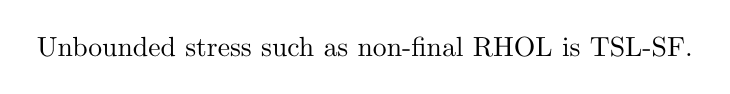
\begin{tikzpicture}
	\node<4> at (3,0) {\alert{Unbounded stress such as non-final RHOL is TSL-SF.}};
	\end{tikzpicture}
\end{frame}

\section[Alternative accounts]{Alternative accounts}

\begin{frame}{An alternative account}
    \textbf{Strother-Garcia et al. (2016):} Unbounded stress as Conjunction of Negative and Positive Literals (CNPL) with enriched strings
    \vskip 2em
    \center
    $
    G_{RHOL} = \sigma \wedge \acute{\sigma} \wedge \neg\acute{L}\sigma \wedge \neg H\acute{\sigma}
    $
\end{frame}

\begin{frame}{CNPL, TSL, TSL-SF, and other accounts}
    \vskip 1em
	\hspace*{1pt}\makebox[\linewidth][c]{%
	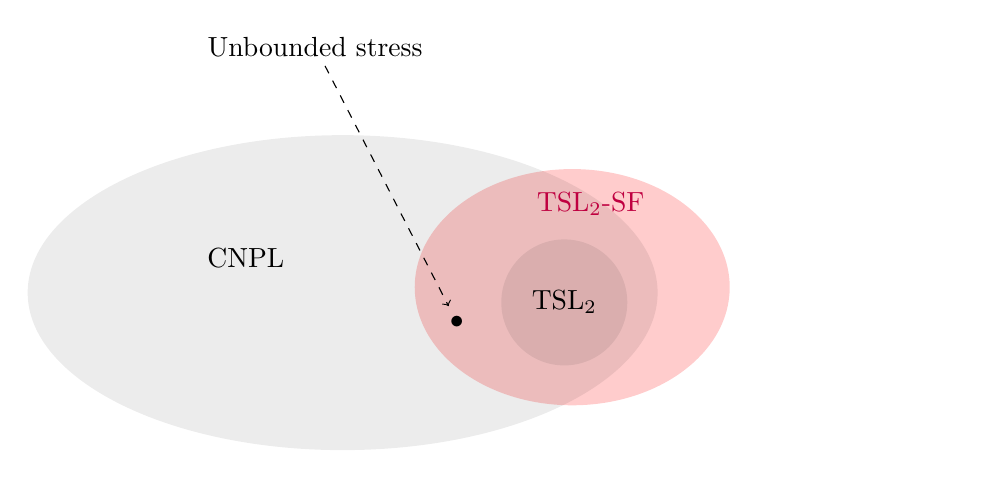
\begin{tikzpicture}
	\begin{scope}[blend group=multiply]
		%\fill[red!30!white] ( 90:1.5) circle (2); 
		\fill[lightgray!30!white] (240:1.3) ellipse (4 and 2); 
		\fill[lightgray!30!white] (330:2.5) circle (0.8);
		\fill<2->[red!20!white] (335:2.5) ellipse (2 and 1.5);
		%\fill<3->[green!20!white] (350:2.2) ellipse (2.5 and 2.7);
		%\fill<4->[orange!20!white] (340:3.2) ellipse (3 and 2); 
	\end{scope}

	%\node at ( 90:2)    {Typography};
	\node at (200:2) {CNPL};
	\node at (330:2.5) {TSL$_{2}$};
	\node<2-> at (360:2.5) {\textcolor{purple}{TSL$_{2}$-SF}};
	%\node<3-> at (37:2.5) {TSL$_{3}$};
	%\node<4-> at (355:5.5) {SS-TSL};
	%\node<4-> at (350:6.2) {(De Santo 2016)};
	\node at (345:6.2) {\phantom{(De Santo 2016)}};
	\node (A) at (0.8,-1.5) {$\bullet$};
	%\node {$\bullet$};
	\node (B) at (-1,2) {Unbounded stress};
	\draw [->, dashed] (B) -- (A);

	%\node [font=\Large] {\LaTeX};
	\end{tikzpicture}}
\end{frame}

\begin{frame}{CNPL, TSL, TSL-SF, and other accounts}
    \vskip 1em
	\hspace*{1pt}\makebox[\linewidth][c]{%
	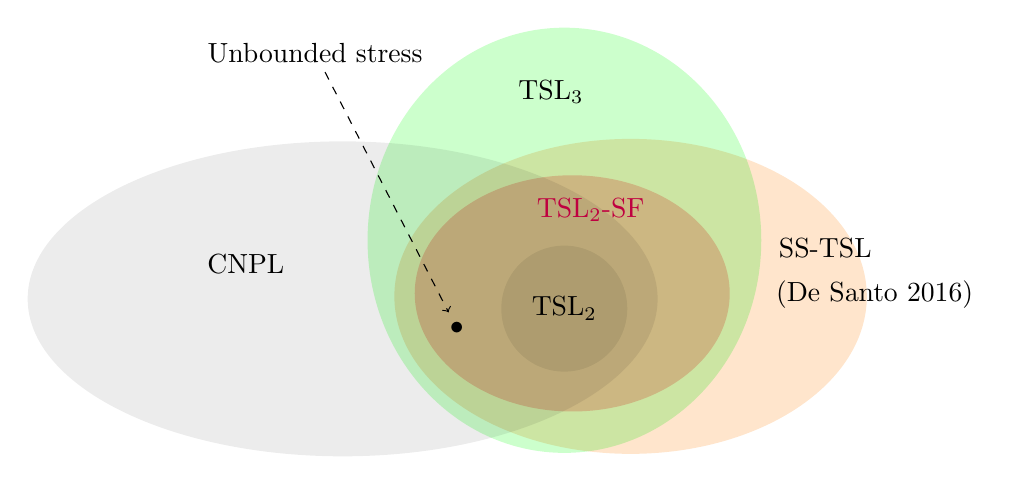
\begin{tikzpicture}
	\begin{scope}[blend group=multiply]
		%\fill[red!30!white] ( 90:1.5) circle (2); 
		\fill[lightgray!30!white] (240:1.3) ellipse (4 and 2); 
		\fill[lightgray!30!white] (330:2.5) circle (0.8);
		\fill[red!20!white] (335:2.5) ellipse (2 and 1.5);
		\fill<2->[green!20!white] (350:2.2) ellipse (2.5 and 2.7);
		\fill<3->[orange!20!white] (340:3.2) ellipse (3 and 2); 
	\end{scope}

	%\node at ( 90:2)    {Typography};
	\node at (200:2) {CNPL};
	\node at (330:2.5) {TSL$_{2}$};
	\node at (360:2.5) {\textcolor{purple}{TSL$_{2}$-SF}};
	\node<2-> at (37:2.5) {TSL$_{3}$};
	\node<3-> at (355:5.5) {SS-TSL};
	\node<3-> at (350:6.2) {(De Santo 2016)};
	\node at (345:6.2) {\phantom{(De Santo 2016)}};
	\node (A) at (0.8,-1.5) {$\bullet$};
	%\node {$\bullet$};
	\node (B) at (-1,2) {Unbounded stress};
	\draw [->, dashed] (B) -- (A);

	%\node [font=\Large] {\LaTeX};
	\end{tikzpicture}}

	\begin{itemize}
		\item CNPL and TSL(-SF) are two incomparable formal classes.
		\item However, TSL-SF has the advantage of staying closer to the hypothesis that phonological patterns are TSL\@.
	\end{itemize}
\end{frame}


\section*{Conclusion}

\begin{frame}{Conlcusion: Unbounded Stress is TSL-SF}
\begin{itemize} 
	\item TSL-SF makes structural features of syllables available in tier projection and substring evaluation.
	\item This expands the expressivity of TSL and accommodates unbounded stress patterns like non-final RHOL\@.
\end{itemize}
\end{frame}

\begin{frame}{References}
\footnotesize
\begin{hangparas}{.25in}{1} 
\textbf{De Santo, A.} 2016. {\em A Game of Tiers: Exploring the Formal Properties of TSL Languages}. Ms., Stony Brook University.\\ 
\textbf{Hayes, B}. 1976. {\em A Metrical Theory of Stress Rules}. Doctoral Dissertation, MIT.\\
% \textbf{Hayes, B}. 1995. {\em Metrical Stress Theory: Principles and Case Studies}.\\
% \ \textbullet \ \textbf{Heinz, J.} 2011. Computational phonology --- part I: Foundations. {\em Language and Linguistics Compass 5}(4), 140-152. 
\textbf{Heinz, J.} 2014. Culminativity times harmony equals unbounded stress. In {\em Word Stress: Theoretical and Typological Issues}, 255-275.\\
\textbf{Heinz, J.} 2016. {\em The computational nature of phonological generalizations}. Ms., University of Delaware. \\ 
\textbf{Jardine, A.} 2014. Computationally, tones are different. {\em Under review with Phonology}.\\
%\textbf{Jardine, A.} 2014. Computationally, tones are different. {\em Under review with Phonology}. \\
\textbf{McCarthy, J.}, 1979. On stress and syllabification. {\em LI 10}(3), 443-465. \\
\textbf{Strother-Garcia, K., Hwangbo, H. J., \& Heinz, J.} 2016. {\em Characterizing and learning unbounded stress patterns with a restricted logic and enriched strings}. AMP 2016 abstract.\\
\end{hangparas}
\end{frame}


\begin{frame}{Appendix 1: suprasegment vs. segment}
    \begin{itemize}
    	\item Jardine (2014): Suprasegmental phonology is more powerful than segmental phonology.
  		\vskip 1em
    	\item e.g., \textbf{First-Last Harmony}(unattested) (Heinz 2016): Word-initial and word-final sibilants agree in anteriority, but word-medial sibilants may disagree.
    \end{itemize}
    \vskip 1em
		\renewcommand{\arraystretch}{1.2}
		\centering
		\small
		\begin{tabular}{c|c}
			\hline
			well-formed  & ill-formed \\
			\hline
			simasas & \textesh imasas \\
			soke\textesh us & soke\textesh u\textesh \\
			\textesh akemi\textesh & sakemi\textesh \\
			\textesh usome\textesh & \textesh usomes \\
			\hline
		\end{tabular}
\end{frame}

\begin{frame}{Appendix 1: suprasegment vs. segment}
    \begin{itemize}
    	\item In the current analysis, the computational gap is derived from the limited availability of structure features.
		\item That is, in prosodic phonology the grammar can refer to structural features of syllables, but not in segmental phonology.
		\item This mirrors existing phonological theories where prosodic features such as \textit{stress} play roles only at a later stage of derivation (Hayes 1976).
	\end{itemize}
\end{frame}

\begin{frame}{Appendix 2: Culminativity as TSL-SF}
    \begin{block}{Non-final RHOL is TSL-SF}
        \vskip 0.5em
        \small
        $
        G= \left \langle T = \begin{Bmatrix}
		[\text{+stress}], \\ [\text{+heavy}],\\ [\text{+initial}], \\ [\text{+final}] 
		\end{Bmatrix}
		, \quad S = \begin{Bmatrix}
		\text{$^{*}$[+heavy,+stress,-initial,+final]}, \\ 
		\text{$^{*}$[+light,+stress,-initial]}, \\
		\text{$^{*}$[+heavy,+stress][+heavy,-stress,-final]}, \\
		\text{$^{*}$[+light,+stress][+heavy,-stress,-final]}
		\end{Bmatrix} \right \rangle
        $
		\vskip 0.5em
    \end{block}
    \vskip 2em
    \begin{block}{Culminativity is TSL-SF}
        \vskip 0.5em
        \small
        $
        G= \left \langle T = \begin{Bmatrix}
		[\text{+boundary}], \\ [\text{+stress}] 
		\end{Bmatrix}
		, \quad S = \begin{Bmatrix}
		\text{$^{*}$[+boundary][+boundary]}, \\ 
		\text{$^{*}$[+stress][+stress]}
		\end{Bmatrix} \right \rangle
        $
		\vskip 0.5em
    \end{block}
\end{frame}


\end{document}